\chapter{Diseño}
\section{Prototipado}
El prototipo de una aplicación conforma una versión inicial <<hueca>> de un producto. Es una herramienta fundamental para visualizar conceptos de diseño, funcionalidad y interacción con el usuario en una etapa temprana de desarrollo. Permite una comunicación efectiva entre el equipo de desarrollo y el cliente, haciendo posible la identificación de problemas antes de la implementación del producto, donde un cambio de requisitos es poco costoso, garantizando que la aplicación satisfaga las necesidades y expectativas de los usuarios finales.

En nuestro caso, como técnica de prototipado hemos optado por utilizar \textit{wireframes}. Los \textit{wireframes} son una herramienta de prototipado basados en representaciones visuales simplificadas de la interfaz de una aplicación. En estos se plasma la estructura y disposición de los elementos fundamentales de la aplicación sin añadir detalles decorativos como elementos de diseño gráfico o colores, centrándose en la funcionalidad y navegación de la misma.

En la figura \ref{fig:proto-home} se puede ver el diseño de la página principal de nuestra interfaz. Como vemos en ella se expone la funcionalidad principal de perfilar una colección de usuarios a partir de un archivo. Esta página, está formada por un formulario donde se puede seleccionar el algoritmo de perfilado junto con el fichero que contiene la colección a perfilar. Por otro lado también tiene una barra de navegación en la parte de arriba que se mantendrá para el resto de \textit{wireframes} de la aplicación.

\begin{figure}[H]
  \centering
  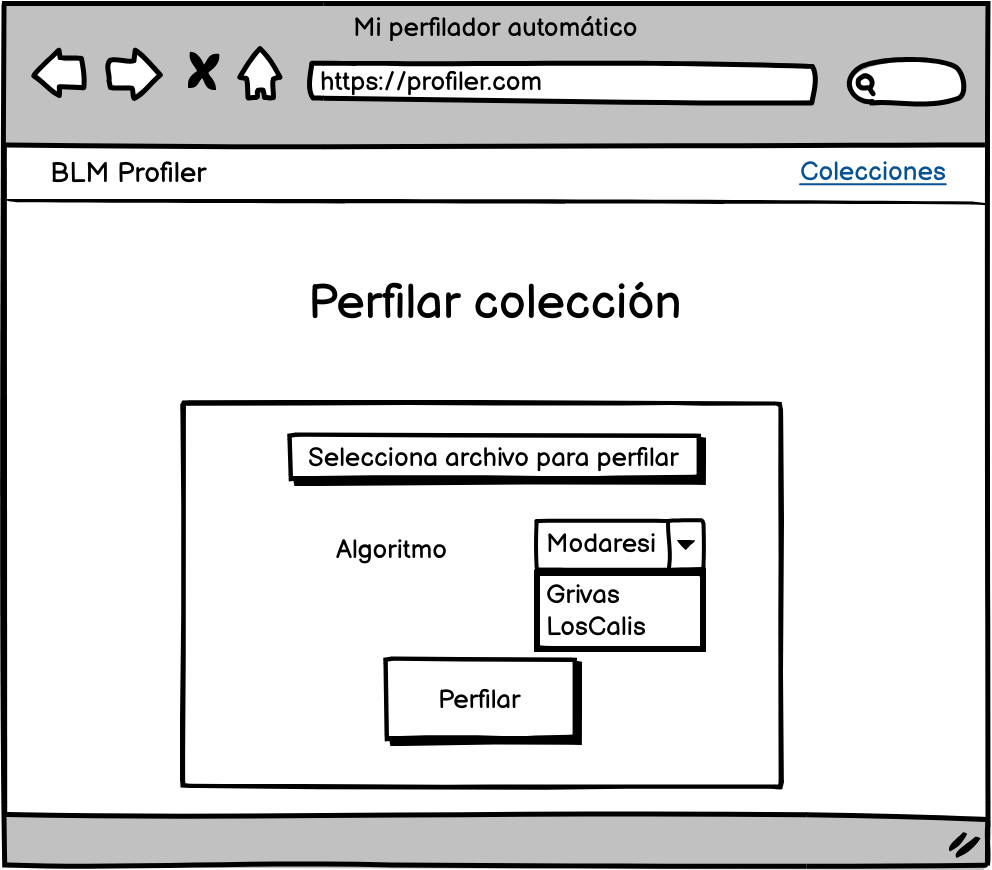
\includegraphics[width=\textwidth]{imaxes/prototipo/home.png}
  \caption{Prototipo de la página principal de la aplicación.}
  \label{fig:proto-home}
\end{figure}

En el caso de seleccionar el enlace <<Colecciones>>, de la barra de navegación, nos iríamos a una página como la de la figura \ref{fig:proto-collections}. En esta se muestra una tabla, ordenada temporalmente, con todas las colecciones de usuarios previamente perfilados de nuestra aplicación, junto a información general sobre cada una como: algoritmo, usuarios totales o fecha de perfilado.

\begin{figure}[H]
  \centering
  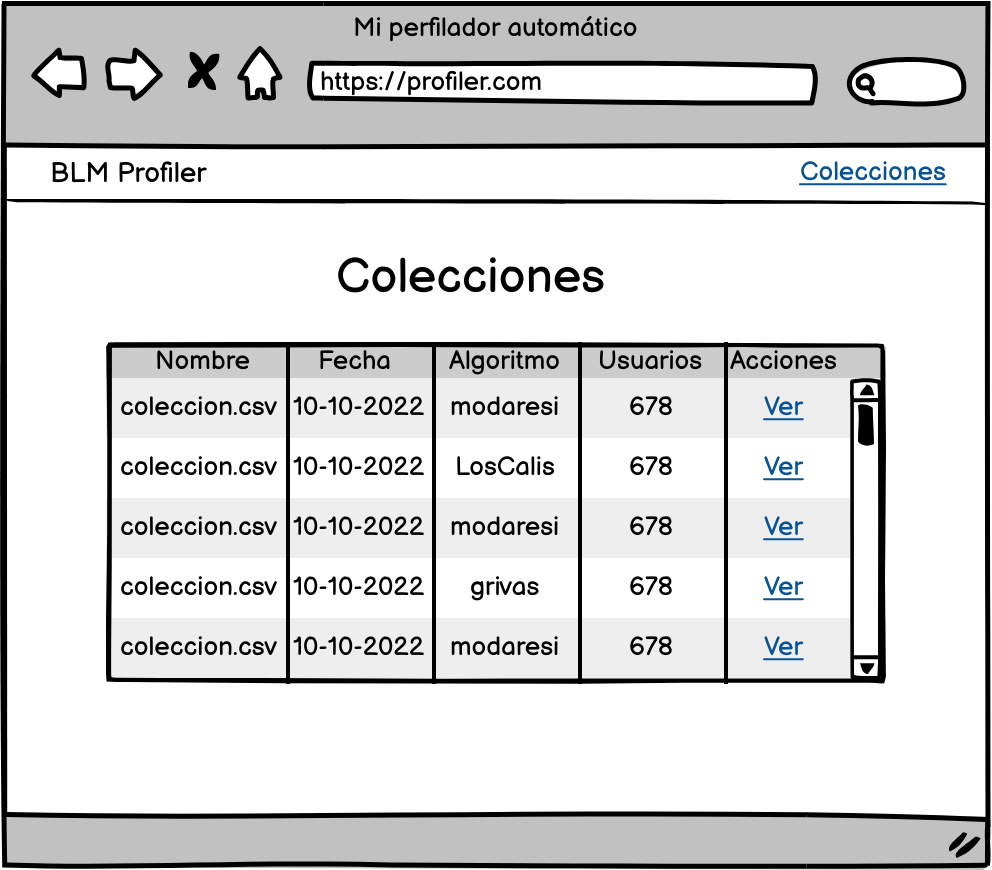
\includegraphics[width=\textwidth]{imaxes/prototipo/collections.png}
  \caption{Prototipo de ver colecciones perfiladas.}
  \label{fig:proto-collections}
\end{figure}

En el caso de seleccionar <<ver>> una colección de la lista de colecciones (\ref{fig:proto-collections}) o tras perfilar una nueva en la página principal (\ref{fig:proto-home}) nos iríamos a la visualización del \textit{dashboard} o cuadro de mando de la colección (\ref{fig:proto-dashboard}). En este \textit{wireframe} se muestran dos gráficas sobre los datos demográficos, edad y género en este caso, de los usuarios perfilados. Además también se muestra una tabla con la lista de usuarios de la colección junto con las predicciones realizadas sobre cada uno y un enlace sobre una muestra de una publicación del mismo. Por otro lado, en la parte de arriba tenemos unos desplegables que nos permiten filtrar los datos de la tabla y gráficas según la categoría elegida; junto con unas tarjetas en las que se muestran detalles generales de la colección.

\begin{figure}[H]
  \centering
  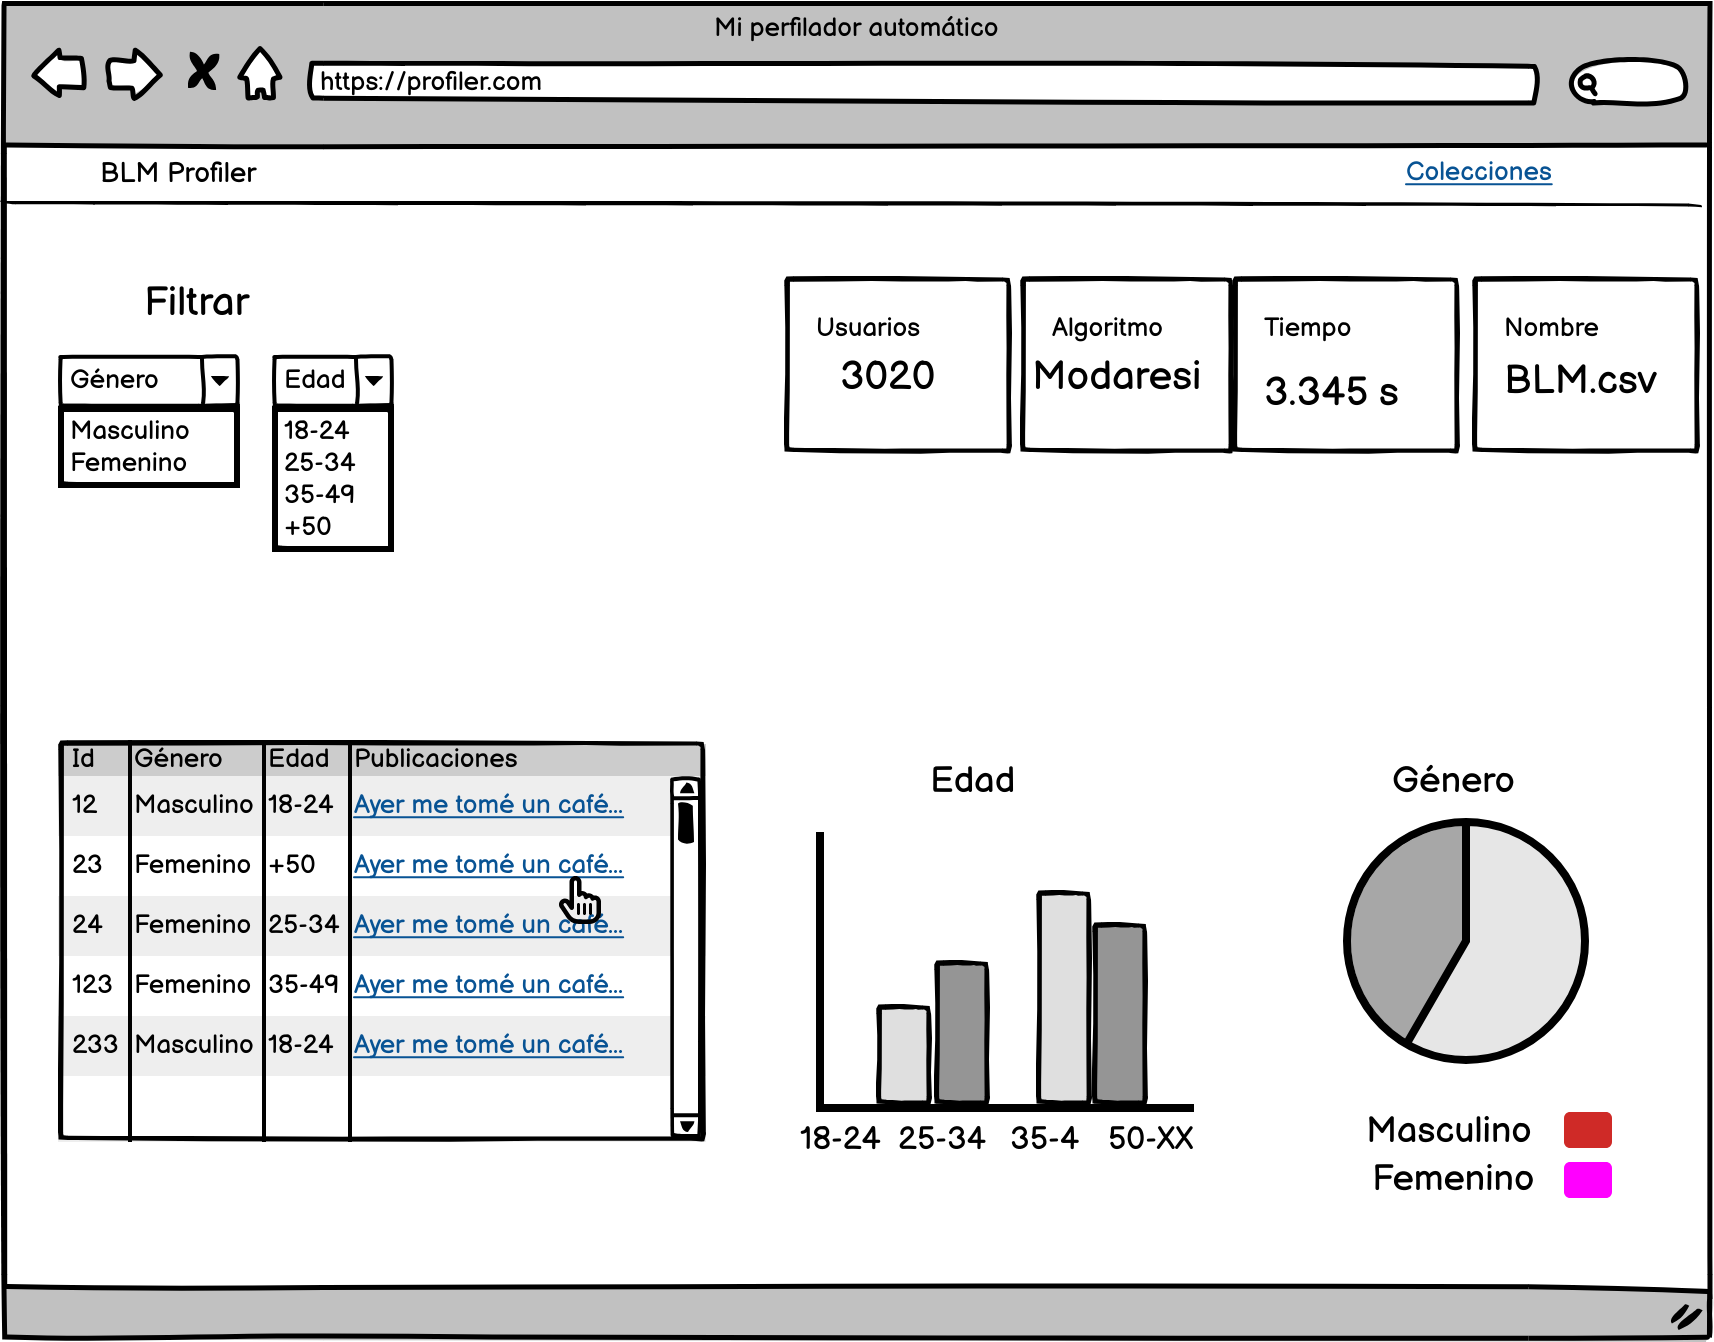
\includegraphics[width=\textwidth]{imaxes/prototipo/dashboard-unfiltered.png}
  \caption{Prototipo del cuadro de mando de la aplicación.}
  \label{fig:proto-dashboard}
\end{figure}

En el caso de seleccionar algún filtro en el \textit{dashboard} se añadiría al mismo una lista, como la de la figura \ref{fig:proto-dashboard-filtered}, con aquellos seleccionados donde se podrían quitar de nuevo estos. Y se mostrarían las modificaciones en los gráficos y lista.

\begin{figure}[H]
  \centering
  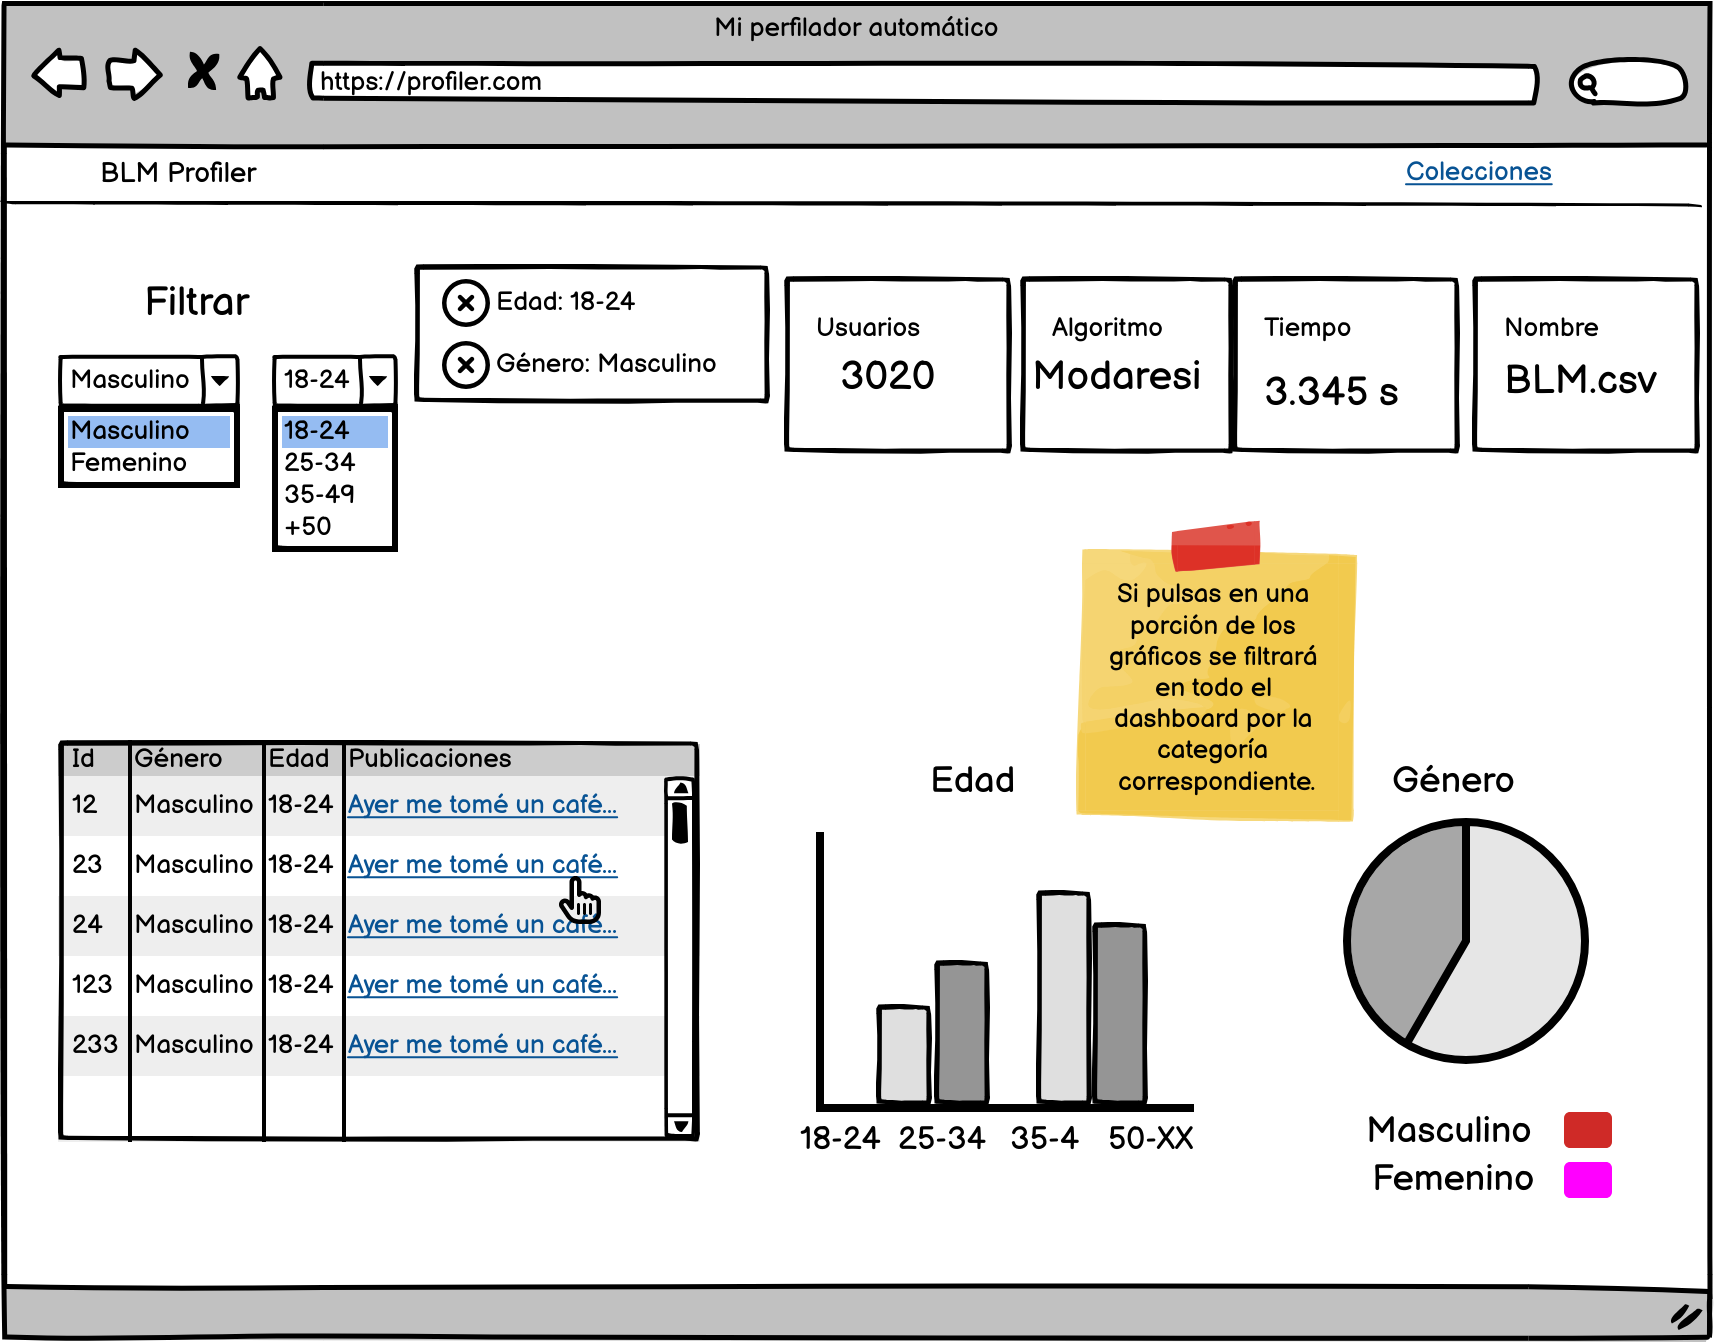
\includegraphics[width=\textwidth]{imaxes/prototipo/dashboard-filtered.png}
  \caption{Prototipo del cuadro de mando al especificar filtros sobre edad y género.}
  \label{fig:proto-dashboard-filtered}
\end{figure}

Por último, al seleccionar el enlace de la publicación de un usuario del \textit{dashboard}, se navegaría hasta la última página de nuestra web, donde se podría ver en detalle las publicaciones del usuario seleccionado junto con sus datos generales. Además, esta tendría un botón para volver al \textit{dashboard} de la colección. En el \textit{wireframe} de la figura \ref{fig:proto-info-user} se muestra la disposición de la misma.

\begin{figure}[H]
  \centering
  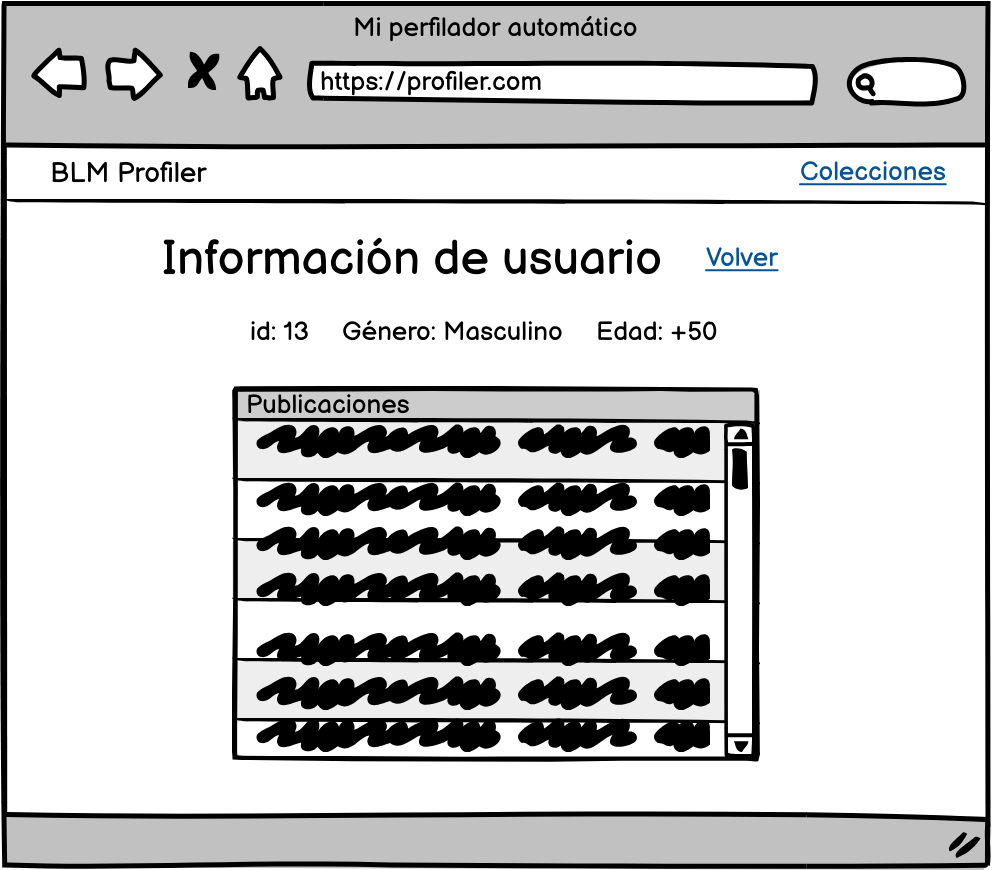
\includegraphics[width=\textwidth]{imaxes/prototipo/info-user.png}
  \caption{Prototipo de ver información de usuario en detalle.}  \label{fig:proto-info-user}
\end{figure}

\section{Arquitectura}
El diseño de la arquitectura de una aplicación es un aspecto de vital importancia para cumplir con los requisitos tanto funcionales como no funcionales de la misma. Dada la naturaleza ágil de la metodología seguida, la arquitectura del sistema ha ido evolucionando durante el desarrollo del mismo, pasando de un diseño más sencillo a uno más complejo. Por este motivo, en este apartado se describirá el diseño final de la arquitectura propuesta.

En nuestro caso, como se puede ver en la figura \ref{fig:diagrama/arquitectura} hemos seguido una arquitectura cliente-servidor distribuida o en n-capas, donde el servidor está dividido en servidor web, servidor de aplicación y servidor de datos. El servidor web es el que aloja la aplicación web SPA, que su vez está divido en interfaz de usuarios y capa de acceso a servicios. El servidor de aplicación se encarga de exponer la API REST que ejecuta la lógica de negocio de la aplicación y el acceso a datos\footnote{Y de comunicarse con el micro-servicio de perfilado como se comenta más adelante.}. Por último, el servidor de datos es el encargado de almacenar los datos de la aplicación. 

\begin{figure}[H]
  \centering
  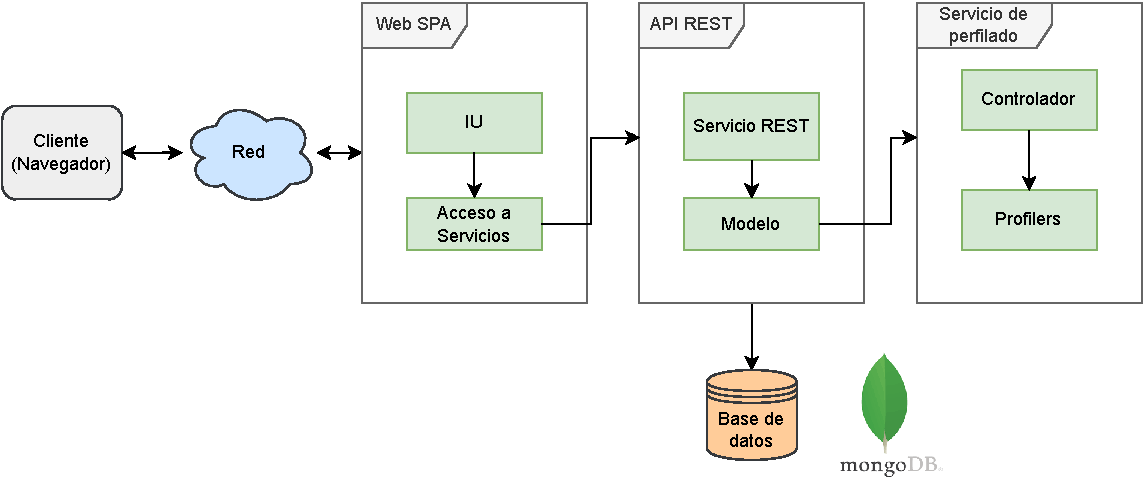
\includegraphics[width=\textwidth]{imaxes/diagramas/arquitectura.pdf}
  \caption{Diagrama de la arquitectura global del sistema.}  \label{fig:diagrama/arquitectura}
\end{figure}

Además se puede ver que existe un servidor adicional, que se podría definir como un micro-servicio, cuya única funcionalidad es la de ejecutar los algoritmos de perfilado sobre los datos de usuarios que le envíe la API REST y devolver estos perfilados. Por lo tanto, la el servidor de la aplicación también actúa como cliente de este servicio. \footnote{La decisión de separar este servicio del resto del <<backend>> se tomó inicialmente debido a la dificultad de hacer la migración de los algoritmos existentes a una versión actual de python como se comentará en el capítulo de desarrollo, sin embargo, este enfoque tiene otros beneficios importantes que se comentan a continuación.}

La decisión de tener esta arquitectura distribuida en varias capas tiene varias ventajas:
\begin{itemize}
    \item Para empezar, se favorece la escalabilidad del sistema RNF-5. El hecho de tener servidores distintos para <<frontend>>, <<backend>> y el micro-servicio de perfilado permite que se puedan escalar horizontalmente estos de forma selectiva. Esto es importante porque el micro-servicio de perfilado representa la carga más significativa del sistema en cuanto a recursos computacionales y tiempo, lo que la convierte en un posible cuello de botella para el funcionamiento general del mismo. Por otra parte, el servidor web es el que menos recursos computacionales consume.
    \item Por otro lado, se favorece la mantenibilidad y extensibilidad del software (RNF-2). El hecho de tener las distintas capas desacopladas posibilita el poder extender o reemplazar cualquiera de ellas sin necesidad de hacer un cambio en las demás\footnote{Este hecho se alinea con unas buenas prácticas de ingeniería, cumpliendo con un principio de diseño fundamental como es el abierto-cerrado.}. Un ejemplo de esto sería añadir un cliente móvil además del web, añadir otra API que consumiera el micro-servicio de perfilado, o incluso extender este último para dar soporte a nuevos algoritmos o mejoras de rendimiento. De igual forma esta separación nos permite elegir el lenguaje de programación o tecnología más adecuada para la implementación de cada capa.
    \item Por último, otra ventaja de este enfoque sería el aumento de fiabilidad del mismo (RNF-3). El fallo en cualquier capa no implica que el resto no puedan seguir funcionando.
\end{itemize}
\subsection{<<Backend>>}
Como ya se ha comentado el <<backend>> está dividido en dos capas: servicios y modelo que a su vez se podría dividir en lógica de negocio y acceso a datos. Para la implementación de estas capas se han seguido diferentes patrones de diseño muy comunes en el desarrollo de este tipo de aplicaciones, como pueden ser el uso del patrón fachada para exponer la funcionalidad de los servicios, el uso de DTOs para la validación y serialización de los datos, la implementación de DAOs con operaciones CRUD para acceder a la base de datos o el modelado de la conexión a la base de datos como un \textit{singleton}. En la figura \ref{fig:diagrama/api} se puede ver el diagrama de clases del <<backend>>.

\begin{figure}[H]
  \centering
  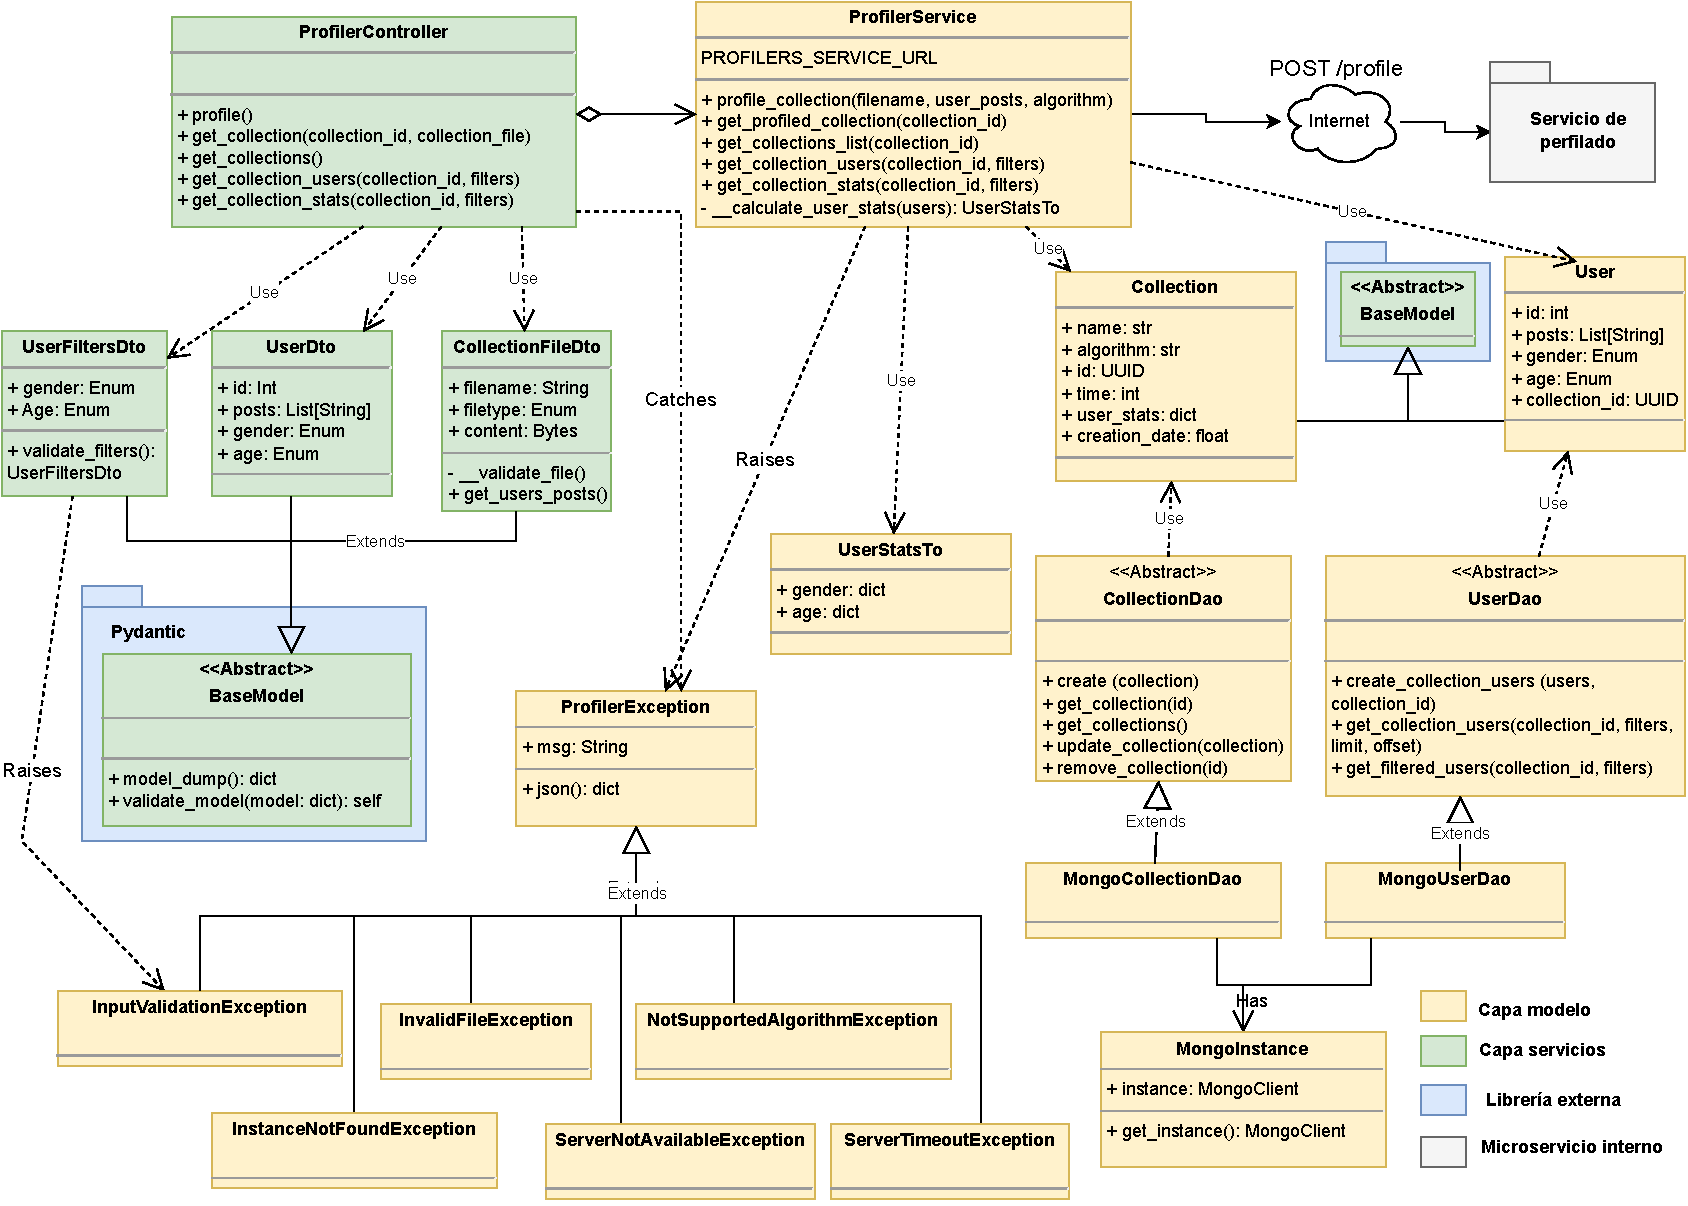
\includegraphics[width=\textwidth]{imaxes/diagramas/backend-classes.pdf}
  \caption{Diagrama de clases final del API REST del sistema.}  \label{fig:diagrama/api}
\end{figure}

\subsection{Micro-servicio de perfilado}
En cuanto al micro-servicio de perfilado se puede comentar que también se ha seguido un enfoque REST, con un único endpoint de entrada, para la comunicación con el <<backend>>. En el diagrama de la figura \ref{fig:diagrama/micro-servicio} se puede ver la estructura de este micro-servicio.
\begin{figure}[H]
  \centering
  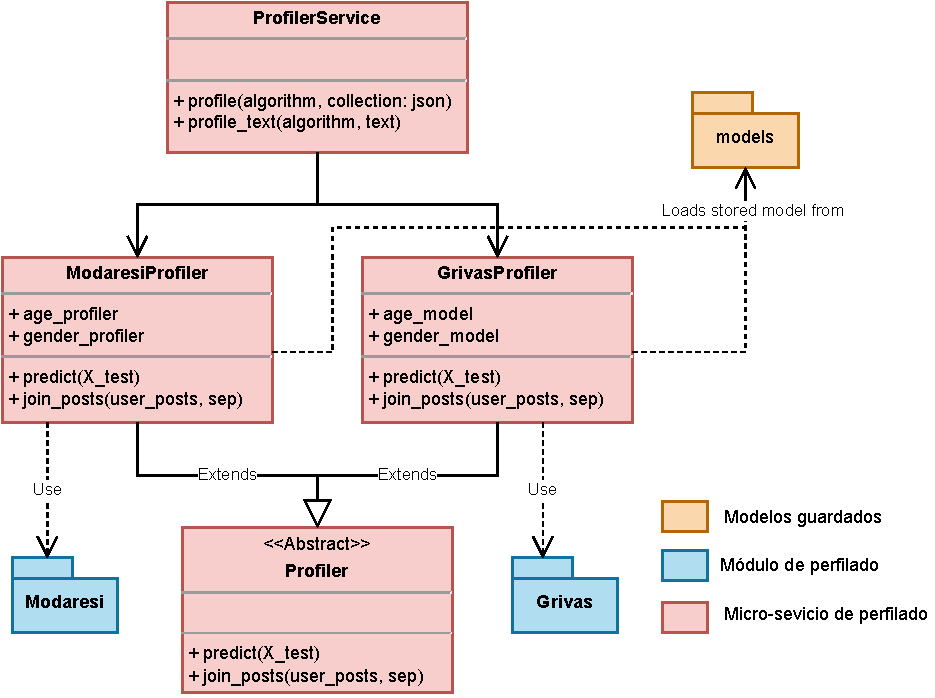
\includegraphics[width=\textwidth]{imaxes/diagramas/profiler-service.pdf}
  \caption{Diagrama de clases final del micro-servicio de perfilado.}  \label{fig:diagrama/micro-servicio}
\end{figure}
En el mismo se muestra que las clases que implementan los \textit{profilers} cargan los modelos y pipelines de preprocesado de un módulo llamado <<models>> donde se encuentran todos aquellos modelos necesarios ya entrenados y listos para el perfilado de los algoritmos.

Estos modelos guardados tienen dependencias con los módulos de perfilado, que se ven color azul en el diagrama, que son aquellos que contienen el código para el preprocesado y creación de los modelos de AA. Sin embargo, como son módulos de autores externos adaptados para el proyecto se decidió no mostrar su estructura en el diagrama de clases.

% \subsection{<<Frontend>>}